\subsection{Communications}
\label{sec:communications}

This section describes the top-level design.% Key details can be found in appendix \ref{ap:communications}.

\subsubsection{Selection process}
The selection criteria for a communications protocol were:
\begin{itemize}
	\item The number of devices supported: Systems supporting less than 93 devices were excluded.
	\item Raw data rate: Systems with a raw data rate of less than $\SI{128.32}{\kilo\bit}$ were excluded.
	\item Physical implementation: 
	\begin{itemize}
		\item Connector requirements: Systems with protocol or implementation specific connectors were excluded.
		\item Noise immunity: Systems without in-built noise immunity and error-checking were excluded.
		\item Ease of cabling installation and maintenance: Multi-drop systems were favoured.
		\item Supported topology: Systems that support multiple topologies were preferred.
	\end{itemize}
\end{itemize}

\subsubsection{Master to Daughterboards} 
Given the timing constraints, number of devices and environmental conditions, the evaluation process identified CAN bus and I2C as suitable communications systems.
CAN was chosen primarily due to its differential signalling mechanisms providing inbuilt noise immunity and upper protocol support. 

\subsubsection{CAN Transceiver Selection}
Although the microcontroller has hardware support for the CAN protocol, it does not have the hardware to physically drive the CAN bus lines.
Therefore, a NCV7344 CAN transceiver IC was selected to perform these actions.
It runs off the same $\SI{5}{\volt}$ rail as the microcontroller and is able to withstand the $\SI{105}{\degreeCelsius}$ temperature requirements.

\subsubsection{CAN Bus Physical Implementation}
Separate cabling is used for data communications to meet the timing and signalling requirements of $\SI{1}{\micro\second}$ and $\SI{100}{\micro\second}$.

30-AWG ribbon cable is used for reliability and ease of installation and maintenance.
Using this will mean the bus is not broken if a daughterboard is removed, while still meeting the timing requirements.
Additionally, there is a greater range of 10 conductor options (compared to 8, 6 or 4 way) which also provides for dual bus expansion options.
Strain relief is also provided with the chosen connector system.
Figure \ref{fig:data_cable} depicts the arrangement of data signals to provide maximum noise immunity and cable reversal protection.
Note that there are two CAN bus lines that are selectable via a solder jumper on the PCB.
\begin{figure}[H]
	\centering
	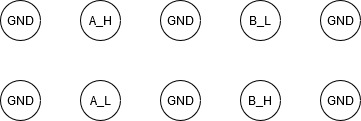
\includegraphics[width=0.4\textwidth]{data_cable}
	\caption{The 10-way data cable with two CAN buses.}
	\label{fig:data_cable}
\end{figure}

30AWG nonilly nominally supports 270kHz for full skin depth.	Actual cable uses 7 strands of 38AWG (nominally 1750kHz for full skin depth).
	Characteristic impeedance is 138 ohms balenced velocity factor of 74 with propagation of 4.53 nano seconds.
	The chosen a cable has slightly higher impeedance to achieve higher velocity factor, knowing that the bus is near end and far end terminated to 120 ohms. This presents 130 ohms in parallel.)

\subsubsection{Master to Data Logger}

The master-board must also connect to a data logger via some means of electrically isolated connection.
After some consideration surrounding the cost of fiber-optic links and their suitability to the thermal environment, an RF solution was chosen.
The 802.11 protocol was chosen for its ubiquity and suitability for purpose.
The 113990816\footnote{\url{https://www.digikey.co.nz/product-detail/en/seeed-technology-co-ltd/113990816/1597-113990816CT-ND/6194658}} from Seeed Technology Co., Ltd is a surface mount component that supports 802.11b/g/n and temperatures of up to $\SI{125}{\degreeCelsius}$.
The only consideration would be the electrical noise produced by the apparatus but this could be reduced by physically locating the master-board away from the high voltage components.
